\documentclass[12pt]{beamer}

%%%%%%%%%%%%%%%%%%%%%%%%%%%%%%%%%%%%%%%%%%%%%%%%%%%%%%%%%%%
%%%%%%%%%%%%%%%%%%%%%%%%%%%%%%%%%%%%%%%%%%%%%%%%%%%%%%%%%%%


\usepackage[orientation=portrait]{beamerposter}
	\usepackage{amsmath, amssymb}
	\usepackage{microtype}
	\usepackage{empheq}
	\usepackage{siunitx}
	\usepackage{dsfont}

	\usepackage{tikz}
	\usetikzlibrary{patterns,arrows,decorations.pathreplacing,hobby}
	\usepackage{graphicx}
\usepackage{natbib}
\usepackage{fontspec}
\setsansfont{Futura}

\usetheme{Berlin}      % or try Darmstadt, Madrid, Warsaw, ...
\usecolortheme{rose} % or try albatross, beaver, crane, ...
%\usefonttheme{serif}  % or try serif, structurebold, ...
\setbeamertemplate{navigation symbols}{}
\setbeamertemplate{caption}[numbered]

	\newcommand{\cit}{\textbf{[$\blacksquare$] }}

\renewcommand{\maketitle}{%
	\begin{center}%
		\Huge\inserttitle\\[5mm]%
		\Large\insertauthor\\[5mm]%
		\Large\insertinstitute%
	\end{center}%
	\vspace*{-1ex}%
}

\geometry{
  hmargin=2.5cm, % little modification of margins
}

\setlength{\paperwidth}{24in}
\setlength{\paperheight}{36in}
\setlength{\textwidth}{\paperwidth}
\setlength{\textheight}{0.9\paperheight}
\setbeamersize{text margin left=0.5cm,text margin right=0.5cm}

% beamer definitions

\makeatletter
\definecolor{lightblue}{RGB}{33,140,168}
\definecolor{crimson}{RGB}{218,61,73}
\definecolor{cream}{RGB}{250, 245, 245}
\definecolor{clay}{RGB}{207, 190, 180}

\setbeamercolor{normal text}{fg=black,bg=white}

\setbeamercolor{block body}{fg=black, bg=lightblue!20!white}
\setbeamercolor{block title}{fg=white, bg=lightblue!60!black}


\setbeamercolor{alerted text}{fg=crimson}


\setbeamercolor{example text}{fg=crimson!50!black}
\setbeamercolor{block body example}{fg=black, bg=cream!80!gray} 
\setbeamercolor{block title example}{fg=white, bg=crimson} 

\setbeamercolor{structure}{fg=cream}

\setbeamercolor{background canvas}{bg=cream, parent=normal text}
\setbeamercolor{background}{parent=background canvas}

\setbeamercolor{palette primary}{fg=cream!40!white,bg=crimson!80!black}
% \setbeamercolor{palette secondary}{use=structure,fg=structure.fg!100!green}
% \setbeamercolor{palette tertiary}{use=structure,fg=structure.fg!100!green} 

\makeatother

%%%%%%%%%%%%%%%%%%%%%%%%%%%%%%%%%%%%%%%%%%%%%%%%%%%%%%%%%%%
%%%%%%%%%%%%%%%%%%%%%%%%%%%%%%%%%%%%%%%%%%%%%%%%%%%%%%%%%%%

\title{Characterizing Computational Techniques for Experimentally Feasible Non-Local Evolution of Two-Qubit Systems}
\author{Shankar Balasubramanian\hspace{1em} Didi Chang-Park\hspace{1em} Kyle Herndon\hspace{1em} Zane Rossi}
\institute{TJHSST Modern Physics and Optics Lab}
\date{9 June 2015}

\begin{document}
\centering
	\begin{frame}{\maketitle}
		\begin{columns}
			\begin{column}{.45\textwidth}
				\begin{exampleblock}{Adaptive Algorithm Theory}
	Adaptive algorithms thrive on the idea that, in a relatively smooth space, in order to find the optimal solution, following one's nose can work. There are many ways in which this `greed' or `intuition' can be implemented. adaptive algorithms, as evidenced by their names, attempt to mimic the process of evolution by the mechanisms of mutation and natural selection. A set of mathematical objects dubbed \emph{organisms}, each containing some set of data, are subjected to tests against some metric depending on the organism's features \cit. This is considered one \emph{generation}, and the best organisms of each generation are bred together (by some deterministic algorithm) and mutated to compete in the next generation.

	In preparation for performing a process like the one described, we take three major steps.
	
	To begin, the degrees of freedom of the system should be analyzed, as these will function as the dimensions of the search space. During this process, the degrees which are less pertinent to a solution's fidelity should be identified and their relative mutation amplitude and frequency altered accordingly.

	Next, the mutations assigned to each degree of freedom will be designed so as to best approach a (hopefully) global extrema in the search space. In general, more volatile mutations will be given to the more effective degrees of freedom, and all mutations will decrease in magnitude and frequency as the number of generations increases \cit. 

	Finally, we need determine the method by which the best organisms of each generation are bred (combined in a way that may retain traits of both.). Note that there is no guarantee under any binary operation that the resulting object will have the same advantages assigned to the parent objects. In the case of well-defined and relatively smooth systems, this breeding will often resemble a sort of average, and the child will often perform similarly to the parents. 

	With these in mind, we can visualize the process as a sort of traversal of a complex multidimensional search space. This will give some heuristic for the arguments for convergence.

%\begin{figure}[htpb]
%	\centering
%	\begin{tikzpicture}[scale=0.75, use Hobby shortcut]
%
%	% main bounding shape
%	\draw[ultra thick, closed=true, dash pattern=on 6pt off 6pt] (2.5,4.5) .. (3.3,6.5) .. (5,7.5).. (7.5,7.9).. (10,7.5).. (11,6.5).. (11,4.5) ..(8.5,2).. (6,3.5).. (3,2).. (2.5,4.5);
%
%	%interior grid
%	\begin{scope}
%		\clip[closed=true] (2.5,4.5) .. (3.3,6.5) .. (5,7.5).. (7.5,7.9).. (10,7.5).. (11,6.5).. (11,4.5) ..(8.5,2).. (6,3.5).. (3,2).. (2.5,4.5);
%
%		\draw[step=1,gray,thick] (0,0) grid (15,15);
%	\end{scope}
%
%	% organism paths
%	\draw[ultra thick, color=lightblue] (4.5, 4.5) -- (6.5, 4.5);
%	\draw[ultra thick, color=crimson, dash pattern=on 0.2cm off 0.2cm] (4.5, 4.5) -- (6.5, 4.5);
%	% yeah, that's right, I just did that (dashed overlay)
%	\draw[ultra thick, -latex, color=lightblue] (6.5, 4.5) -- (7.5,4.5) -- (7.5,3.5) -- (8.5,3.5) -- (8.5,7.5);
%	\draw[ultra thick, -latex, color=crimson] (6.5, 4.5) -- (6.5,6.5);
%
%	% organism circle
%	\fill[fill=lightblue] (4.5,4.5) circle (0.4cm);
%
%	% organism symbol and arguments
%	\node[right] at (-0.5, 9) {\large{$\Theta:\;$ \small{\sc{Arguments}}}};
%	\draw (-0.5, 8.5) -- (4, 8.5);
%
%	\node[right] at (-0.5, 6) {$\{A_i\}\;\;\{B_i\}$};
%	\node[right] at (-0.5, 5) {$\{t_i\}\;\;$};
%	\node[right] at (-0.5, 8) {$H:\;$ \small{\sc{Constant}}};
%	\node[right] at (-0.5, 7) {$N:\;$ \small{\sc{Constant}}};
%
%
%
%	\end{tikzpicture}
%	\centering
%		\caption{
%		This is a simplification; the organism being tested is represented by the circle in blue, while the search-space (which has a defined metric represented by the grid) surround it. The paths of different color shown represent the non-deterministic paths possible as the organism mutates and is bred with other successful organisms. The actual space being searched is not two- but many-dimensional.
%		}
%	\end{figure} 
\end{exampleblock}
\begin{exampleblock}{Arguments \& Degrees of Freedom in the Test Organism}
	%%%%%%%%%%%%%%%%%%%%%%%%%%%%%%%%%%%%%%%%%%%%%%%%%%%%%%%


	For the adaptive algorithm process described, each organism, denoted $\Theta$, is given a set of arguments which define it and serve as its characteristics. For our purposes, these can be further divided into \emph{constants} and \emph{mutables}. 

	Among the constants, we have $H$, a set Hamiltonian that is easy to generate, and is used in every free evolution between LO. It does not change in each simulation, across all organisms, and across all generations. We also have $N$, which defines the number of LO-FE pairs for all organisms in a given simulation. None of these variables is subject to the mutation protocol that defines adaptive algorithms. 

	\begin{equation}
		\underbrace{  (A_1\otimes B_1)e^{-i H t_1}\cdots(A_{N}\otimes B_{N})e^{-i H t_{N}}}_{N}
	\end{equation}

	The mutable data contains all of the sets. This includes the set of $A_i$, which are unitary operators on the first particle, the set of $B_i$, which are unitary operators on the second particle, and the set of $t_i$, which are the discrete durations for each FE, and have the constraint of summing to a particular value.
	
	In any effective adaptive algorithm, the structure of the search space must be known. This allows both a functioning and efficient algorithm. In this scenario, the dimension of the space depends on the step number $N$ in a linear fashion. We begin with a local operation, $A$, which is of the form

	\begin{equation}
		\beta \cdot \sigma 
		= 
		\begin{pmatrix}
			\beta_0 + \beta_3    &    \beta_1 - i \beta_2\\[3mm]
			\beta_1 + i \beta_2  &    \beta_0 - \beta_3
		\end{pmatrix}
	\end{equation}

	This appears to have four degrees of freedom, one for each element of $\beta$. However, there is an implicit restraint given the unitarity of the LO, we may recognize this as an exponentiation of a linear combination of the pauli-matrices. 

	\begin{equation}
		A^{\dagger}A = \mathds{1} \implies A = \mathds{1}\cos{|\beta'|} + (\beta' \cdot \sigma) \sin{|\beta'|}
	\end{equation}

	And we recognize this form as being equivalent to the specification of a single point by a new vector $\beta'$ on the three sphere. Thus $A$ is also equivalent to 

	\begin{equation}
		exp\{\beta' \cdot \sigma\} = exp\{\beta'_1 \sigma_1 + \beta'_2 \sigma_2 + \beta'_3 \sigma_3 \}
	\end{equation}

	This gives six degrees of freedom for each pair of local operations. We also note that given variability in the discrete FE times, we would be given $N-1$ more degrees of freedom (the restriction is due to their sum being defined). All considered,  we are searching a $6N$-dimensional space for every $N$-family.



				\end{exampleblock}
							\end{column}
							
			\begin{column}{.45\textwidth}
				\begin{exampleblock}{Results}
						    \begin{figure}[htpb] 
		\centering
			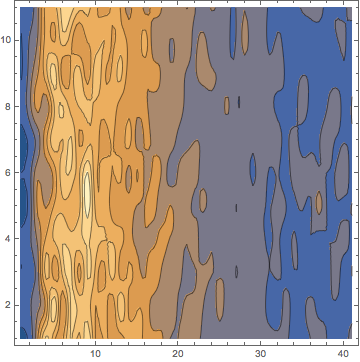
\includegraphics[scale=2]{efficiency_plot.png}
		\centering
		\caption{This plot shows the fidelity of the best organism in a ten-organism set after $100$ generations with respect to mutation chance and mutation magnitude. The vertical axis, when the value is multiplied by $0.1$, gives the chance in any generation for one of the angles defining an organism to be mutated. The horizontal axis, when multiplied by $0.025$, gives the mutation magnitude (this ranges between $0$ and $1$ radian(s)). The plot shows clear correlation between mutation magnitude and organism success.}
        \label{fig:effplot}
	\end{figure}

				\end{exampleblock}
				\vspace{1em}
							\end{column}
	
		\end{columns}
	\end{frame}

%%%%%%%%%%%%%%%%%%%%%%%%%%%%%%%%%%%
%% Half slides %%%%%%%%%%%%%%%%%%%%%%%%%%%	
	\begin{frame}
		\begin{columns}
			\begin{column}{.45\textwidth}
				\begin{exampleblock}{Background}
					The ultimate goal of Control Theory is the ability to arbitrarily manipulate the state of an ensemble of qubits. In the context of quantum computation, this problem is reduced further: basic quantum gates allow for modular systems \cite{bremner}. However, the generation of these gates is non-trivial, and the arbitrary Hamiltonian is, in general, not readily constructible. Often one will wish to achieve a specific unitary evolution operator or gate $U$ corresponding to the solitary time evolution of a Hamiltonian $H$. When $H$ may not be engineered easily, the evolution can be achieved in other ways \cite{bremner} , often involving the use of local operations (LO), repeated measurements on the system \cite{bennett}, along with standard Hamiltonian-driven evolution drawing from some collection (possibly a one element collection) $H_1, H_2, \cdots, H_n$, all of which \emph{can} be lucratively generated.

	In the simplest case, a two particle system, the Hamiltonians involved may contain non-local terms, usually corresponding to particle-particle interactions. This paper will propose a framework for taking the general non-local Hamiltonian \cite{bennett} 
	\begin{equation}
	H = A \otimes \mathds{1} + \mathds{1} \otimes B + \sum_{ij} M_{ij}\,  \sigma_i \otimes \sigma_j
	\end{equation}
	and interspersing its non-local part's evolution with LO to achieve a desired $U$. It is only the non-local part of the Hamiltonian which must be studied, and through decomposition of this piece into its canonical form, and some insight into Lie Theory, we are able to formulate a computational approach \cite{haselgrove}. Devising a scheme to generate a $U$ from a collection of available operators and Hamiltonians has direct applicablity to a variety of problems, but cannot be done purely analytically on a massive scale, thus making a computational method necessary.
				\end{exampleblock}
				\vspace{1em}
								\begin{block}{References}
					\bibliographystyle{plain}
				\bibliography{ref}		
				\end{block}
			\end{column}
		\end{columns}
	\end{frame}	
\centering


\end{document}